\documentclass[12pt]{article}

\usepackage[utf8]{inputenc}
\usepackage[T1]{fontenc}
\usepackage[a4paper,left=2cm,right=2cm,top=2.5cm,bottom=2cm]{geometry}
\usepackage{amsfonts}
\usepackage{amsmath}
\usepackage{amssymb}
\usepackage{amsthm}
\usepackage{natbib}
\usepackage[english]{babel}
\usepackage{hyperref}
\usepackage{cleveref}
\usepackage{color}
\usepackage{dsfont}
\usepackage{enumitem}
\usepackage{graphicx}
\usepackage{pifont}
\usepackage{tabto}
\usepackage[all]{xy}
\usepackage{nomencl}
\usepackage{wrapfig}
\usepackage{tikz}
\usepackage{tkz-euclide}
\usetikzlibrary{positioning, fit, calc, shapes, arrows, matrix, shapes.misc, snakes, intersections}

\theoremstyle{plain}% default
\newtheorem{thm}{Theorem}[section]
\newtheorem{lem}[thm]{Lemma}
\newtheorem{prop}[thm]{Proposition}
\newtheorem*{cor}{Corollary}
\theoremstyle{definition}
\newtheorem{dfnt}{Definition}[section]
\newtheorem{exmp}{Example}[section]
\newtheorem{xca}[exmp]{Exercise}
\theoremstyle{remark}
\newtheorem*{rmq}{Remark}
\newtheorem*{note}{Note}
\newtheorem{case}{Case}
\newtheorem{hyp}{Hypothesis}

\crefname{thm}{theorem}{theorems}
\crefname{lem}{lemme}{lemmes}
\crefname{prop}{proposition}{propositions}
\crefname{cor}{corollaire}{corollaires}
\crefname{dfnt}{definition}{definitions}
\crefname{exmp}{exemple}{exemples}
\crefname{xca}{exercice}{exercices}
\crefname{rmq}{remarque}{remarques}
\crefname{note}{note}{notes}
\crefname{case}{case}{cases}
\crefname{hyp}{hypothese}{hypothese}

\newcommand{\ncref}[1]{\cref{#1} "\nameref{#1}"}
\newcommand{\Ncref}[1]{\Cref{#1} \Nameref{#1}}

%\makenomenclature

\begin{document}

%\title{On Teichmuller theory and Thurston earthquake flow}
%\author{Etienne Bonnafoux}
%\subtitle{A closer look at the expenses}
%\date{Mars-Juny 2020}

\begin{titlepage}
	\centering
	
\includegraphics[width=0.15\textwidth]{Image/Sorbonne.png}\par\vspace{1cm}
	{\scshape\LARGE Sorbonne Université \par}
	\vspace{1cm}
	{\scshape\Large Master Thesis\par}
	\vspace{1.5cm}
	{\huge\bfseries Teichmuller theory and Thurston Earthquake flow\par}
	\vspace{2cm}
	{\Large\itshape Bonnafoux Etienne\par}
	\vfill
	supervised by\par
	Carlos \textsc{Matheus}

	\vfill

% Bottom of the page
	{\large \today\par}
\end{titlepage}

\newpage

%\maketitle

\newpage

\tableofcontents
\newpage

\section{Introduction}
\input{Introduction.tex}
\newpage

\section{Notations}
\printnomenclature
\begin{tabular}{ll}
  $\mathcal{ML}$ &  measured lamination  \\
  $\mathcal{MF}(S)$ & space of all equivalence classes of measured foliations. \\
  $\mathcal{T}_g$ & Teichmuller space of surface of genus $g$ \\
  $\mathcal{P}^1 \mathcal{M}_g$ & Product of $\mathcal{T}_g$  and $\mathcal{MF}(S)$ quotiented by the modular group. \\
$\mathcal{GC}(S)$  & the space of geodesic currents \\
\end{tabular}

\nomenclature{$\mathcal{MMMM}$}{mMmM}

\newpage

\section{Teichmuller Theory}
Nous commencerons dans cette section par donner quelques définitions pour introduire la théorie des espaces de Teichmuller.

\begin{dfnt}{Espace de Teichmuller}
Soit $S$ une surface de genre $g$, un marquage de $S$ est un couple $(X,f)$ formé d'une surface de Riemann $X$ et d'un homéomorphisme préservant l'orientaion $f:S \to X$.
Sur l'ensemble des marquages de $S$, nous pouvons faire une relation d'équivalence $(X_1,f_1) \sim (X_2,f_2)$ si il existe $\alpha : X_1 \to X_2 $ tel que $f_2 \circ \alpha \circ f_1^{-1}$ soit un homéomorphisme de $S$ préservant l'orientation et isotope à l'identité.
L'espace des marquages quotienté par la relation s'appelle l'espace de Teichmuller et est noté $\mathbb{T}_g$
\end{dfnt}

\begin{rmq}
Si $g \geq 2$, pour toute courbe simple fermée $\alpha$ de $S$, il existe une unique géodésique fermée de $X$ librement isotope à $f(\alpha)$. Nous noterrons $L_{\alpha}(X)$ sa longeur hyperbolique et nous prenons la topologie la plus faible sur $T_g$ qui rendent ces fonctions continues.
\end{rmq}

\begin{dfnt}{Espace des modules}
On appele groupe modulaire le groupe des homéomorphisme préservant l'oriention de $S$ quotienté par ceux isotope à l'identité.Nous notterons ce groupe $Mod_g$.
Il agit de façon discrète sur $T_g$ et l'espace quotient est appelé espace des modules et est noté $\mathbb{M}_g$
\end{dfnt}

Il est naturel de ce demander à quoi ressemble ces espaces.

\begin{dfnt}{Dehn twist}
Soit $\gamma$ une courbe simple et fermée. Il existe un voisinage tubulaire de $\gamma$ noté $A$ homéomorphe à $[0;1] \times S^{1}$.
On définit le Dehn's twist comme l'homéomorphisme qui vaut l'indentité hors de $A$ et vaut $(t,s) \mapsto (t,e^{2i \pi t} s)$ sur $A$.
\end{dfnt}

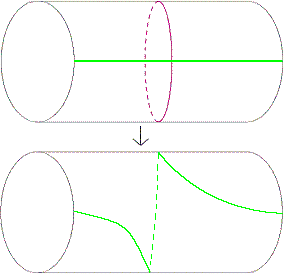
\includegraphics[width=6cm]{Image/Dehn_twist.png}

\begin{rmq}
Le théorème de Lickorisk affirme que le groupe modulaire est engendré par ces Dehn's twist et que plus précisément on peut choisir $2g+1$ générateurs \cite{Lickorish1964AFS}.
\end{rmq}

\begin{dfnt}{Feuilletage}
Un feuilletage mesuré est un feuilletage de la surface dont chaque arc porte une mesure. Ainsi la mesure d'un arc $\gamma$ ne dépent que de la feuille d'arrivé
\end{dfnt}

\begin{dfnt}{Lamination}
Une lamination est un ensemble fermé qui est un union (non nécessairement finie) de géodésiques.
Par chaque point x contenu dans $\lambda$ il ne passe que une seul géodésique.
Nous notterons cet espace $\mathbb{ML}(x)$
\end{dfnt}

\begin{dfnt}{Différentielle quadratique}
Une différentielle quadratique est une section du carré de l'espace tangeant canonique à X. Il s'écrit localement comme $\phi= \phi(z) dz^2$
\end{dfnt}

\begin{rmq}
Si $\phi(p) \neq 0$ on peut trouver une carte contenant $p$ dans laquel $\phi = dz^2$.
Ainsi $\phi$ détermine une métrique plate sur $X$ et un feuilletage $\mathbb{F}$ correspondant aux lignes horizontales.
\end{rmq}

Une différentielle quadratique est dite intégrable si \[
 \| \phi \| = \int_X | \phi | < \infty
\]
Nous notterons $\mathbb{Q}(x)$ l'espace de Banach des différentielles quadratiques intégrables.
%Differentiel quadratique
%Feuilletage
%Lamination
%tremblement de terre
%flot horocycle
%Nombre d'intersection

\newpage

\section{Mirzhakani's Isomorphism}
The aim of this part is to demonstrate the followoing statement

\begin{thm}
There is a measurable conjugacy $F$ between the earthquake flow $(\lambda , X) \mapsto (\lambda, E_{t \lambda}(X))$ on $\mathcal{ML}\times \mathcal{T}_g $ and the Teichmüller unipotent flow action of \[
u_t = \begin{pmatrix} 1 & t \\ 0 & 1 \end{pmatrix}
\]
on the bundle $\mathcal{QD}$ of nonzero quadratic differentials over Teichmüller space $\mathcal{T}_g$ .
\end{thm}

\[
\xymatrix{
  \mathcal{ML}\times \mathcal{T}_g  \ar[r]^{E_t} \ar[d]_F  & \mathcal{ML}\times \mathcal{T}_g \ar[d]^F \\
   \mathcal{QD} \ar[r]_{u_t} & \mathcal{QD}
 }
\]

\subsection{Tightening map}%TODO vériphier l'orthographe

A first coresspondance, found by Thurston, exist between measured foliation and measured lamination. We will mostly follow the paper of Levitt \cite{levittfoliations}.

\begin{dfnt}
We say that two foliations are equivalent if we can pass from one to the other by Whithead (see definition below) moves or isotopy (homeomorphism isotopic to the identity).
\end{dfnt}


\begin{dfnt}
Given a measure foliation, an critical segment $\gamma$ is an arc between two singularities along a leaf which is not a simple closed curve.
There is a map $f$ homotopic to the identy that collapse $\gamma$ to a point $x$ and is identity outside a neighboorhood of $\gamma$ which contain no other singularity .  Doing so we reduce the number of singularities of the foliation and if the extremoties of $\gamma$ are singularities of order $k_1$ and $k_2$, $x$ is now a singularity of the new foliation of order $k_1+k_2-2$.
\end{dfnt}


\begin{center}
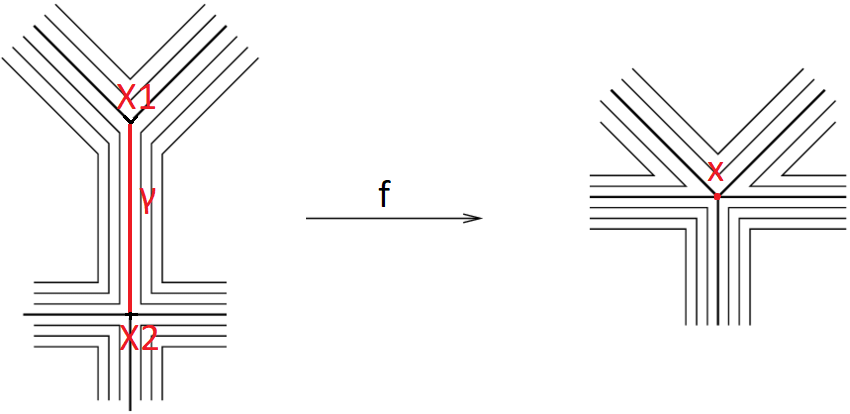
\includegraphics[width=10cm]{Image/Whitehead-move-collapsing-or-creating-an-arc-joining-two-singular-points.png}
\end{center}

\begin{thm}
Let $X$ be a closed orientable hyperbolic surface and $\mathcal{F}$ a foliation. There is a canonical geodesic lamination $\gamma(\mathcal{F})$ associated to $\mathcal{F}$. If $\mathcal{F}$ and $\mathcal{F}'$ are associated foliation then $\gamma(\mathcal{F})= \gamma(\mathcal{F}')$. In the opposite direction given a geodisic lamination $\gamma$, one can find a foliation $\mathcal{F}$ such that $\gamma(\mathcal{F})=\gamma$ and it's unique up to equivalence.
\end{thm}
%TODO mettre le recouverment universel
\begin{dfnt}
A \emph{tranverse curve} is a simple closed curve $C$ which is never tangent to $\mathcal{F}$ and contain no singularity of $\mathcal{F}$.
\end{dfnt}

\begin{rmq}
Since $\mathcal{F}$ contain only saddle singularities, $C$ cannot be contractible, therefor $C$ is isotopic to a simple closed geodesic.
\end{rmq}

We will work on the universal cover of $X$, which is the Poincaré disc $\mathbb{D}$ with circle "at infinity" $\mathbb{S}$. We call $p:X \to \mathbb{D}$ the universal projection.
$\mathcal{\tilde{F}}$ is $p^{-1}(\mathcal{F})$.

We will say that a foliation follow the (*) condition if the following is true:
\begin{center}
If $f_1$ and $f_2$ are two compact homotopic leaves then all leaf in the open annulus between them  is also compact.
\end{center}

\begin{lem}
Let $h$ be a leaf of $\mathcal{\tilde{F}}$. Each end of $h$ converge to a point of $S$; the two point at infinity cannot be the same
\end{lem}

\begin{proof}
First, we should notice that the behavior of leaf at infinity do not change if we take an equivalent foliation. Indeed a homeomorphism $\phi$ on a compact fundamental domain isotopic to the identy can be extend to an homeomorphism $\tilde{\phi}$ on $\mathbb{D}$ such that $dist(x,\tilde{\phi}(x)) \leq K$. This implie that $\tilde{\phi}$ extend es the identity on the boundary $\mathbb{S}$.

\smallbreak
Then given a leaf $h$ of $\mathcal{\tilde{F}}$, we take a half leah $h_0$. If $p(h_0)$ is compact or spiral toward a compact leaf of $\mathcal{F}$ then the first part of the lemme is imediate.

\smallbreak
Otherwise, $p(h)$ meet a transverse curve $C$ infinitely often. With an isotopie we can take $C$ to be a geodesic. Now $h_0$ can meet a connect component of $\tilde{C}=p^{-1}(C)$ only one time. Otherwise there will be a disk bound by an arc of $\tilde{C}$ and an arc of $h_0$, which is impossible considering the transversity of $C$ and that $\mathcal{F}$ have no $1$-type singularities.

\smallbreak
Now every compact of $\mathbb{D}$ meet a finite number of connected components of $\tilde{C}$ so the limit set of $h_0$ must be on $\mathbb{S}$. This limit set is connected and non empty. Moreover it should not contains any end of a connected component of $\tilde{C}$. But the ends of connected components of $\tilde{C}$ are dense in $\mathbb{S}$ as $\tilde{C}$ is the image of a geodesic by $\pi_1(X)$. This show the first point of the lemma.

\smallbreak
The second assertion is clear if $p(h)$ is compact or if it meet a transverse curve $C$ at least twice since then every connected componnents of $\tilde{C}$ separate the end of $h$.

\smallbreak
Otherwise $p(h)$ spiral toward two compact leaf $f_1$ and $f_2$. If $f_1=f_2$ and the two end point of $h$ are the same then there will be a singularity that would not be a saddle. $f_1 \neq f_2$ is impossible since $\mathcal{F}$ follow the condition (*).
\end{proof}

\smallbreak
We can now associate to every leaf $h$ a geodesic $\gamma(g)$ by joining the endpoint. Then $\tilde{\gamma(\mathcal{F})}= \cup_{h \in \mathcal{F}} \gamma(h)$ is a disjoint union of geodesic invariant by $\pi_1(X)$. We have to show that this set is closed to conclued that we have a lamination.

\begin{lem}
$\tilde{\gamma(\mathcal{F})}$ is closed in $\bar{\mathbb{D}}$
\end{lem}

\begin{proof}

Let $g_n=\gamma(h_n)$ be a sequence of geodesics in $\tilde{\gamma(\mathcal{F})}$ converging to a geodesic $g$. We want to show $g \in \tilde{\gamma(\mathcal{F})}$. We can suppose that all the $g_n$ are distinct of $g$ and are all on the same side.

\smallbreak
Let $L$ be the limit set in $\bar{\mathbb{D}}$. For all leaf $m$ in $\tilde{\mathcal{F}}$, we call $\bar{m}$ the closure of $m$
 by adding the two end point in $\mathbb{S}$. Then $L$ meet at least one connected component of $\bar{\mathbb{D}} \\ \bar{m} $. As the end points of all leaf of $\tilde{\mathcal{F}}$ is a dense subset of $\mathbb{S}$, $L$ contain a leaf $h$. Taking a half-leaf $h_0$, we want to show that the end point is the same as one of $g$.

\smallbreak
A first case is if there is a simple closed curve $C$  transverse to $\mathcal{F}$ which meet $p(h_0)$ infinitely often. If $h_0$ does not converge to the corresponding point at infinity then there would be a connected component of $p^{-1}(C)$ that contains the point of infinity of $h_0$ but does not contain the point of infiny of $h_n$ which is impossible for large $n$.

\smallbreak
A second case is if $p(h_0)$ spirals toward a compact leaf, then closed leaf close to $p(h_0)$ also spirals toward the same compact leaf. Then $h_0$ converges to one of the points at infiniy of $g$ which is a point at inifinity of $h_n$ fot $n$ large.
\smallbreak

Finally if $p(h)$ is compact then $p(h_n)$ spirals toward it for large $n$, therefore $\gamma(h)$ and $g$ have one point in common at infinity. If the second was different, by applying a transformation leaving $\gamma(h)$ invariant (but no $g$), we would separate $h$ from the leaves $h_n$, and it is a contradiction.
%TODO finir la preuve : réciproque
\end{proof}

Now we want to exhib an inverse construction which take a lamination $\lambda$ and give a foliation $\mu$. To do this we still consider $\tilde{\lambda}$ in the universal cover. We will suppose that every complementary region is a ideal polygon.
%TODO expliquer pourquoi cette situation est générique

We can built a skeleton that it compose of edge between vertex and a choosen point in the center. After building the skeleton for every polygon we fill the complementary region which will be between four edge by line between the two vertex.

This map is often called the "collapsing" map and its inverse the "tightening" map.
%
\begin{figure}[h!]
\centering
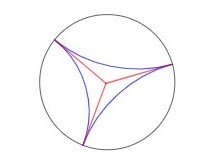
\includegraphics[width=6cm]{Image/CollapsingTightening.jpg}
\caption{In red the skeleton of the ideal triangle in blue, Image from \cite{wright2018mirzakhani}}
\end{figure}

The measure we put on this foliation is uniform on every region between four edges of the skeleton.
%TODO ca semble foireux
\subsection{Correspondance between foliations and quadratic differentials}

For a quadratic differential $q$, one can define two measured foliations, the horizontal $h(q)$ and the vertical $v(q)$ corresponding in locate coordinate to $Re(z)$ and $Im(z)$. This give a map two the pair of foliation but it is not the subjectif, we should restrict ro the image.
Define $\Delta = {(\alpha,\beta):i(\alpha,\gamma)=i(\beta,\gamma)=0, \text{ for some }\gamma \in \mathcal{MF}}$. $\Delta$ contain the diagonal $(\alpha,\alpha)$ and is kind of "fat" diagonal.

\begin{lem}
For any $q \in \mathcal{QD}$, $(h(q),v(q)) \notin \Delta$
\end{lem}

\begin{thm}
The map $q \mapsto (h(q),v(q))$ define a homeomorphism $\mathcal{QD} \to \mathcal{MF} \times \mathcal{MF} \backslash \Delta$
\end{thm}

\subsection{Shear Cordinate}
%NOTE 238 Kerchoff une homotopy sur le disque qui respecte un groupe fushian s'étend sur le bord résultat de Nielsen

Finally there is a map that, given a hyperbolic structure $X$ and a lamination $\lambda$ create a measured foliation which is transverse to $\lambda$.

For simplicity we will ask that $\lambda$ is a maximal lamination i.e. if $\tilde{\lambda}$ is the pre-image of $\lambda$ in the universal cover $\mathbb{D}$, $\mathbb{D}\backslash \tilde{\lambda}$ is made of ideal triangle. We will first work in this triangles minus a region on the center, then give a measure in this foliation, and finnally show that ot is a homeomorphism.

So in one the ideal triangle, given two side we can draw an arc prependicular with the this two sides, which is the intersection of the ideal triangle with the circle tangent to the boundary of $\mathbb{D}$ in the common extremity the two arc chosen. Then by rescaling by a factor $r \in [0;1]$ and doing the same procedure for the two other pair we get a foliation in the ideal triangle minus a locus in the center.


\begin{figure}[h!]
\centering
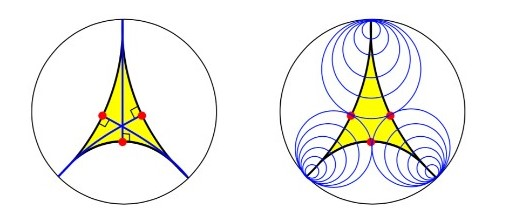
\includegraphics[width=10cm]{Image/FoliationTri.jpg}
\caption{Image from \cite{Martelli2016AnIT}}
\end{figure}

Then we can find a full foliation by pitching the resulting.

We have a natural transverse measure to this foliation. For an arc in one ideal triangle of the lamination we can project it along the leaf of the foliation to asegment in the edge of the ideal triangle, the length of the arc will be the length of the segment. As the leaf are horocycle circle based on the same point, it will not depend of which side we choose to project. Then given an arbitrally arc we decompose it along the ideal triagle it meet.

We want to shwo that this construction is reversable, that is given $\mu \in \mathcal{MF}_\lambda $, the set of foliation transverse to the lamination, we can
construct $X \in \mathcal{T}_g$ whose horocycle foliation is $\mu$.

The idea is that, if we already know $X$, the lamination $\lambda$ can be lift to $\tilde{lambda}$ which is invariant of $\Gamma$ the fushian group of $X$. But we can built $\tilde{lambda}$ only with the information given by $\mu$.

We will note $\tilde{\mu}$ the preimage of $\mu$ in $\mathbb{D}$. If we consider two triangles $T_1$ and $T_2$  that are complementary region of $\tilde{\lambda}$ and we suppose we take a segment $A$ in a leaf of $\tilde{\mu}$ that goes to an edge of $T_1$ to $T_2$. We name $v_1$ and $v_2$ the two vectors with footprint in the edge and tangent to them. Then there is a Moebuis transformation $S$ which take one to the other. With one more information, the "shear", we can place $T_2$ on $\mathbb{D}$, according to the position of $T_1$

\begin{figure}[h!]
\centering
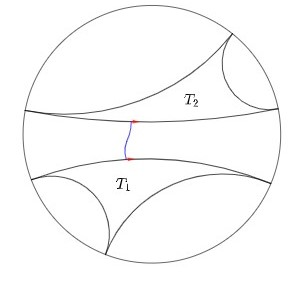
\includegraphics[width=6cm]{Image/Foliation.jpg}
\caption{Image from \cite{wright2018mirzakhani}}
\end{figure}

Indeed given only a Moebuis transformation we still have a one parameter families of triangle $T_2$ with an edge generated by $v_2$. To fix this we trace two orthogeodesic comming from the vertex of the ideal triangles facing the considered edges and from the point of intersection in $T_1$ we follow a leaf of the foliation, then when we meet $T_2$ we have to move along the geodesic edge to find the other point of intersection. This lenght is the shear between $T_1$ and $T_2$

\begin{figure}[h!]
\centering
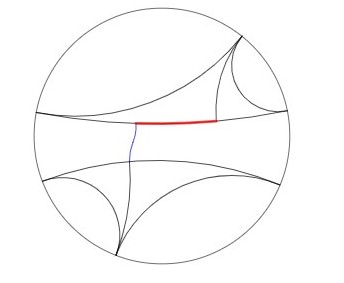
\includegraphics[width=6cm]{Image/Shear.jpg}
\caption{Image from \cite{wright2018mirzakhani}}
\end{figure}

Let $I$ be the set of all triangles in $\mathbb{D}$ that $A$ meet. For each $i\in I$ we can define $v_i^+$ and $v_i^-$ the vectors tangent to the edge of the corresponding triangle at the intersection of the edges and $A$. Note that $I$ is a countable totally ordered but non well ordered set. So if we take $S_i$ the Moebuis transformation which take $v_i^-$ to $v_i^+$, we have to give a meaning of the expression \[
\prod_{i\in I}S_i
\]

\begin{dfnt}
Given a countable totally ordered set of indice $I$ and element $S_i$ in a Banach algebra, we say that $\prod_i S_i$ is well defined and equal to $S$ if for any increasing chain \[
I_0 \subset I_1 \subset ... \subset I
\]
with $\cup_k I_k=I$ we have $lim_{k \to \infty} \prod_{i \in I_k}S_i =S $.
\end{dfnt}

\begin{lem}
For element $s_i$ in a Banach algebra index by a countable totallyordered set, if $\sum \| s_i \| < \infty$, then $\prod(1+s_i)$ is well-defined.
\end{lem}
\begin{proof}
For $1 \leq m \leq n$, we have \[
\| \prod_{i=1}^n(1+s_i)-\prod_{i=1,i \neq m}^n (1+s_i) \| \leq \|s_m \| \| \prod_{i=1,i \neq m}^n (1+s_i) \| \leq \|s_m\| \prod_{i=1}^n (1+\|s_i\|)
\]
Or with the assumption $\sum \| s_i \| < \infty$ we have that $\prod(1+\|s_i\|) \leq C < \infty$, so removing or adding $1+s_m$ produce a change bound by $\|s_m\| C$.
\end{proof}

Now we want to apply this lemma to $S_i - Id$, with $Id$ the identity matrice.

\begin{lem}
For the previous $S_i$, if we note $s_i=S_i - Id$ we have $\sum \| s_i \| < \infty$.
\end{lem}

\begin{proof}
Each $S_i$ is conjugate to a horocycle transformation of time one. The conjugacy is made by a geodesic flow along the edges of the triangle. We can compute \[
\begin{pmatrix} e^{-t/2} & 0 \\ 0 & e^{t/2} \end{pmatrix} = \begin{pmatrix} 1 & 1 \\ 0 & 1 \end{pmatrix} \begin{pmatrix} e^{t/2} & 0 \\ 0 & e^{-t/2} \end{pmatrix} = \begin{pmatrix} 1 & 0 \\ 0 & 1 \end{pmatrix}+ \begin{pmatrix} 0 & e^{-t} \\ 0 & 0 \end{pmatrix}
\]
So the norm of $s_i$ is inversally corrolated to the amount of geodesic flow used in the conjugaison.
Now we can parttion the indice set $I$ into finely many subset $(I_k)$ according to to which spike of the lamination the arc of $A$ cross.
Then for a spike the sum of $\|s_i \|$ where $i \in I_k$ is finite, indeed the distance between two neighbooring crossing is bound below by a constant and so the amount of time we should do the geodesic flow increase at most linerally and finnaly the norm of the $s_i$ should decraese geometrically.
\end{proof}

So we can conclude that there is an unique Moebuis transformation $S$ equal to the meaningfull expression $\prod_i S_i$.

Now we can conclude the proof. There exist, without any hyperbolic structure $X$  topological classes for $\tilde{\mu}$ and $\tilde{\lambda}$. We choose one arbitrary ideal triangle $T_1$ in the lamination. For every other triangle $T_2$, the Moeubuis transformation and the shear are data that can be compute only using the transverse measure of $\tilde{mu}$. So we can place $T_2$, and the other triangle. The closure of this set give the lamination $\tilde{\lambda}$. $\tilde{\lambda}$ will be preserve by a fushian group $\Gamma$ and we will have $X=\mathbb{D}  / \Gamma$.

\newpage

\section{Mixing rate}
\subsection{Mixing proprities of the geodesic and horocyclic flows}

We will first give the behavior of two flows we described before.

\begin{thm}
The ergodic flow and the horocycle flow are mixing.
\end{thm}

\cite{Mcmullen1998HyperbolicM}

\begin{proof}
The step will be in four step, first we will show that the ergodic flow is ergodic, the horocyclic flow is ergodic, the ergodic flow is mixing, finally the horocycle flow is mixing.

\emph{Ergodicity flow is ergodic}

We will look at the time average of a function $f \in L^2$ which is continuous and compactly support. It will be sufficient since this space is dense \[
F(x) = lim_{T \to \infty} \frac{1}{T} \int_0^T f(g_t x)dt
\]
We want to show that $F$ is almost everywhere constant.

Since $F$ depend only of the geodesic $\gamma(a,b)$ which pass at $x$, if $a,b \in S_\infty$ are the two endpoints of $\gamma$, we have $F(a,b)$.
Then as two geodesic with the same forward endpoint are asymptotic, $F$ is a quantity that depend only of asymptotic average, we have that $F$ do not depend of $a$.
But we can reverse the argument to show that if we consider the inverse geodesic, $t \to \infty$, we have that $F$ is also independent of $b$. Hence $F$ is constant almost everywhere and the geodesic flow is ergodic.

\emph{Ergodicity of the horocycle flow}

Now if we take $f \in L^2(X)$ a function invariant under the horocycle flow and of mean zero, we want to show that $f=0$ almost everywhere.
Let $G^t$, $H^s$ and $E^r$ correspond to the operators of the different flows. We have the relation \[
H^s=E^r G^t E^{\pi+r}
\]
where $r \to 0$ as $t \to \infty$. Since $H^s f=f$,we have for any $T>0$,\[
f=\frac{1}{T} \int_0^T E^r G^t E^{\pi+r} f dt
\]
Thus for every $g\ in L^2(X)$ we have \[
<g,f> = \int_X g \frac{1}{T} \int_0^T E^r G^t E^{\pi+r}
\]
As $r \to 0$ then $t \to \infty$ we can show by controlling the difference that \[
<g,f> = lim_{t \to \infty} \int_X g \frac{1}{T} \int_0^T G^t E^{\pi} f dt
\]
Then as we have shown that the geodesic flow is ergodic, we have by Von Neumann ergodic theorem\[
<g,f> = <g,\int_X E^{\pi} f> =0
\]
This conclude the proof that the horocycle flow is ergodic.

\emph{Mixing of the geodesic flow}

We have the relation \[
h^s g^t =g^t h^{s exp(2t)}
\]
Let us take $f_0,f_1 \in C_0(X)$,
we have for small $s$ %TODO rendre ca plus rigoureux
\[
<f_0,g^t f_1 > \equiv <h^{-s} f_0,g^t f_1 >=<f_0 , h^s g^t f_1 >
= <f_0 , g^t h^{s exp(2t)} f_1 > = <g^{-t} f_0 , h^{s exp(2t)}f_1>
\]
Now we have for small $s$, \[
h^{S exp(2t)}f_1 \equiv \frac{1}{S} \int_0^S h^{exp(2t)s} f_1 ds =F_t
\]
and for large t, as the horoclic flow is ergodic \[
F_t = \frac{1}{S} \int_0^S h^{exp(2t)s} f_1 ds \equiv \int_X f_1 = <f_1 , 1 >
\]
So we have \[
<f_0, g^t f_1 > \equiv <g^{-t} f_0, F_t > \equiv <g^{-t} f_0 ,1 ><f_1,1> = <f_0,1><f_1,1>
\]
Which is the mixing of the geodesic flow.

\emph{Mixing of the horocyclic flow}

We use again the relation $h^s = e^r g^t e^{\pi + r}$. \[
<h^s f_0 , f_1 > = < g^t  e^{\pi+r} f_0, e^{-r} f_1> \equiv <g^t e^{\pi} f_0, f_1
\]
for $t$ large (and so $r$ small). By the mixing propity of the geodesic flow, this quantity converges to $<f_0,1><f_1,1>$, and the horocyclic flow is mixing.

\end{proof}


Then we have this elementary corrolary

\begin{cor}
The Earthquake flow is also ergodic.
\end{cor}

\begin{proof}
With the conjugacie of Mirzharani, the earthquake flow is conjugated to the horocycle flow which is ergodic. This propriety is transmitted.
\end{proof}

\subsection{Rate of mixing of this flows}

Then we want to know at which rate the mixing of the geodesic and horocyclic flow happend. Ratner show in 1986 \cite{ratner_1987} that the geodesic flow is exponnetially mixing and the horocyclic flow has a polynomial rate of mixing. She used representation theory.

We will first give some definition before abording the main theorem.

\begin{dfnt}
Let $H$ be a  complexe separable Hilbert space, $U(H)$ the group of all unitary transformation of $H$ onto itself and $T: G \to U(H)$ a unitary representation. We note $T(g)=T_g \in U(H)$.

An element $v \in H$ is called \emph{a $C^k-vector$} for $T$, $k=0,1,...,\infty$ if $g \mapsto T_g(v)$ is a $C^k$-map from $G$ to the Hilbert space.
\end{dfnt}

\begin{rmq}
The space of $C^{\infty}$ vector is dense in H.
\end{rmq}

\begin{dfnt}
If $v$ is a $C^1$-vector of $H$ and $X$ is in the Lie algebra of $G$, the \emph{Lie derivative} $L_X v$ is \[
L_X v =lim_{t \to 0} \frac{T(exp tX)v-v}{t}
\]
\end{dfnt}

Now if $\Gamma$ is a fushian group, $SL_2(\mathbb{R})$ act on the hyperbolic surface with its measure $(X,\mu)$ as seen as $\mathbb{H}/ \Gamma$.
Then it will also act by a representation $\rho$ on $L^2_0(X,\mu)$ the space of zero average function on the surface.

We want to study the decorellation induce by some subgroup of $SL_2(\mathbb{R})$. It will link with this quantity.

\begin{dfnt}
Let $\phi$ and $\psi$ be zero-mean functions in $L^2$, the \emph{matrix coefficient} $C_{\phi,\psi}$ is\[
g \mapsto |<\phi, \rho(g) \psi>|
\]
\end{dfnt}

\begin{rmq}
As the horocyclic flow and the geodesic flow are mixing we have $C_{\phi,\psi}(e_t) \to 0$ and $C_{\phi,\psi}(h_s) \to 0$ for all functions $\phi$ and $\psi$.
\end{rmq}

We can decompose this representation as an integrale of irreductible representation \[
L^2_0(X,\mu)=\int H_\zeta d \nu(\zeta)
\]
With $\rho_{\zeta}$ the representation oh $H_{\zeta}$.

This set of representation decompose in three part. \begin{enumerate}
\item The principal serie
\item The discrete serie
\item The complementary serie
\end{enumerate}

This decomposition is given by the spectrum of the Casimir operator on each $H_\zeta$.
The discrete part of the spectrum is the discrete series, and if $q$ is the iegenvalue, the part $q \geq 1/4$ is the principal series and $q < 1/4$ the complemetary series. This decomposition was studied by Bargmann in \cite{10.2307/1969129}.

So we can decompose $\nu=\nu_p + \nu_d + \nu_c$.

Moreover we now that if $\rho_\zeta$ is in the complementary series, there exist $s=s(\zeta) \in ]0;1[$ such that the representation is isomorphic to the representation $\pi_s$ on the Hilbert sapce \[
\mathcal{H}_s =
\{ f:\mathbb{R} \to \mathbb{C}
, \|f \|^2 = \int_{\mathbb{R} \times \mathbb{R}}
 \frac{f(x) \bar{f(y)}}{|x_y|^{1-s}}dxdy < \infty\}
\]
With the action \[
pi_s \begin{pmatrix}a & b \\c & d \end{pmatrix}f(x)=\frac{1}{(cx+d)^{1+s}}f(\frac{ax+b}{cx+d0})
\]
The representation $rho$ is isolated from the trivial representation if and only if there exist $\epsilon >0$ such that $s(\zeta)<1-\epsilon$ for $\nu_c$ almost every $\zeta$.


The Lie algebra of $SL(2,\mathbb{R})$, is the vector space of $2 \times 2$ matrice with zero trace. A basis for this space is \[
W=\begin{pmatrix} 0 & 1 \\ -1 & 0 \end{pmatrix}, Q=\begin{pmatrix} 1 & 0 \\ 0 & -1 \end{pmatrix}, V=\begin{pmatrix} 0 & 1 \\ 1 & 0 \end{pmatrix}
\]
Which give the Casimir operator on $C^2$ vectors of $SL(2,\mathbb{R})$, \[
\Omega_T = (L_v^2+L_Q^2-L_W^2)/4
\]

If $T$ is irreductible then $\Omega_T$ is a scalar multiple of the identity, i.e. \[
\Omega_T v = \lambda v
\]

for some $\lambda=\lambda(T)\in \mathbb{R}$ and all $C^2$-vectors $v \in H(T)$

If $\Gamma$ is a lattice of $SL(2,\mathbb{R})$, $\Omega_T$ create an operator $\Delta$ on $\Gamma \backslash SL(2,\mathbb{R})$. We call $\Lambda(\Delta)$ its spectrum and
\begin{enumerate}
\item $A(\Gamma)=\Lambda(\Gamma) \cup ]-1/4;0[$
\item $B(\Gamma)=sup A(\Gamma)$
\item $C(\Gamma)= -1 + \sqrt{1+4 B(\Gamma)}$
\end{enumerate}

We can now write the theorem about the decay of correlation.

\begin{thm}
Let $\Gamma$ be a lattice in $SL(2,\mathbb{R})$, $M=\Gamma \backslash G$ and $T$ be the regular representation of $G$ on $L^2 (M, \mu)$. Let $v,w\in K(T,p)$, $p>0$, $<w,1>=0$ and $B(t)=<v,w \circ g_t>$, $C(t)=<v,w \circ h_t>$.
Then there exist $t_0=t_0(\Gamma)>0$ such that for all $|t| \geq t_0$ and some $E,F > 0$
\begin{enumerate}
\item $|B(t)| \leq E( b(|t|))^{\alpha(p)}$
\item $|C(t)| \leq F( b(ln|t|))^{\alpha(p)}$
\end{enumerate}
where

\begin{enumerate}
\item $b(t)=e^{\sigma(\Gamma)}$ if $A(\Gamma) \neq \emptyset$
\item $b(t)=e^{-t}$ if $A(\Gamma) = \emptyset$, $sup(\Lambda \cap ]- \infty; -1/4[) < -1/4$ and $-1/4$ is not an eigenvalue of $\Omega$
\item $b(t)=te^{-t}$ if $A(\Gamma) = \emptyset$, $sup(\Lambda \cap ]- \infty; -1/4[)= -1/4$ or $-1/4$ is an eigenvalue of $\Omega$
\end{enumerate}
and $\alpha(p)$ is
\begin{enumerate}
\item $1$ if $p \geq 3$
\item $\frac{2p}{2p+1}$ if $2 \leq p < 3$
\item $\frac{2p}{2p+3}$ if $1 \leq p < 2$
\item $\frac{p}{p+3}$ if $0<p<1$
\end{enumerate}
\end{thm}

%TODO refaire en dessous

On the other we can make the path backward, by learning information on the representation via the mixing rate of the flow it generates. This way is taken in the appendice B of \cite{2005math.....11614A}.

\begin{dfnt}
Let $G$ be a locally compact $\sigma$-compact group. A continuous unitary
 representation of $G$ is said to have \emph{almost invariant vectors}
 if for every $\epsilon > 0$ and for every compact subset $K \subset G$, there exists a unit vector $V$ such that $\|g*v-v\| < \epsilon$ for all $g \in K$.

 A unitary action which does not have almost invariant vectors is said to be \emph{isolated from trivial representation}.

 If $G$ is a semi-simple Lie group, a representation which is isolated from trivial representation is alos said to have a spectral gap.
\end{dfnt}

With this definition, we can write the following theorem.

\begin{prop}
Let consider a representation of $SL(2,\mathbb{R})$ by a measure presearving action of automorphisms of a probability space. Let $\rho$ be the repesentation associate on $H$ the space of the $L^2$ function with zero averages. Assume there is $\delta \in ]0;1[$ and a dense subset of the subspace of $SO(2,\mathbb{R})$-invariant function $H' \subset H$ consisting of functions $\phi$ for which the correlations $<\phi, \rho(g_t) \time \phi>$, $g_t=\begin{pmatrix} e^t & 0 \\ 0 & e^{-t} \end{pmatrix} $
, decay like $O(e^{- \delta t})$. Then $\rho$ is isolated from the trivial representation.

\end{prop}

\newpage

\section{Example of the once punctured torus}
A torus can not have a hyperbolic structure, it has naturally a flat structure as the quotient $\mathbb{R}^2 / \mathbb{Z}^2$.
This changes when one study the one ponctured torus. It is a torus $S$ where we choose a point $p$ and remove it (or just marked it).

The construction of this object can be done in two manier at least.
For the first construction, one have to choose a hyperbolic octogone where one side have length $0$ and the two other one $l$, then we sew the border of two of this octogone which give a pair of pant. Finally we can glued with a twist $\tau$ to have the one ponctured torus.

A second construction is given by the representation. Given two hyperbolic isomorphism of $\mathbb{H}$ $A$ and $B$ with different fixed point on $\delta \mathbb{H}$ and with $H := ABA^{-1}B^{-1}$ the commutator should be a parabolic element.

A fundamental domaine is given by the following image:


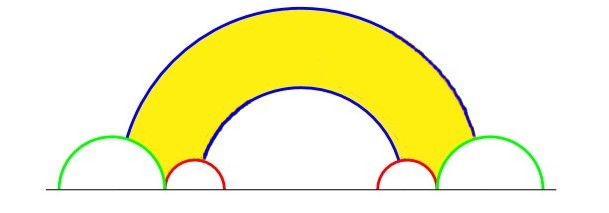
\includegraphics{Image/OnceTorusFundamentalDomaine.jpg}

Given two generators $\alpha$ and $\beta$ of $\pi_1(S)$, two closed curves non homotopically trivial which intersect one, one can parametrize all other lamination.
Indeed a given lamination $\lambda \in \mathcal{ML}$ is determined by the couple $(i(\alpha,\lambda),i(\beta,\lambda))$ where $i(.,.)$ is the geometric intersection number.

We have this useful lemma to estimate the length of the systole function in the Teichmuller space.

\begin{lem}
Pick $\gamma$ a simple closed geodesic, and $X \in \mathcal{T}(S_{1,1)}$, if $X$ has Fenchel-Nielsen coordinate $(L,\frac{p}{q})$ with respect to $\gamma$, where $gcd(p,q)=1$ and $\frac{p}{q} \in ]0;1[$, then \[
C_1(L) e^{\frac{-L}{2q}} < l_{sys}(X) < C_2(L) e^{\frac{-L}{2q}}
\]
where $C_1(L)$, $C_2(L)$ both limits to $4$ when $p$, $q$ are fixed and $L$ goes to $\infty$
\end{lem}

\begin{proof}
Let $R(L)$ be the length of the shortest geodesic arc with endpoints on $\gamma$. We have \[
R(L)= 2 log(coth(L/4))=2 log(\frac{e^{l/2}+1}{e^{l/2}-1})
\]
By the collar lemma. %TODO une référence interne bien sympa
Then if we take $\alpha$ a simple closed curve that intersect $\gamma$, $q$ times exactly, we obtain the following inequality with $a=l_\alpha(X)$ \[
q R(a) < L < q R(a) + \frac{qa}{2}
\]
Reorganizing the termes we have \[
e^{-a/4}tanh(a/4) < e^{-L/2q} < tanh(a/4)
\]
As $a \rightarrow 0$ then $L \rightarrow \infty$
\[
C_1(L) e^{\frac{-L}{2q}} < a < C_2(L) e^{\frac{-L}{2q}}
\]
To complete the proof , we need to show that the length of $\alpha$ is shorter than any other géodesic closed curves, but with the collar lemma there is only one systole whose length goes to $0$ and this is the case for $\alpha$ as $L \rightarrow \infty$. %TODO detailler la preuve

If we don't don any approximation we have \[
2 ln(\frac{1+e^{-L/2q}}{1-e^{-L/2q}}) < a
\]

\end{proof}

\begin{thm} Let $\nu(S_{1,1})$ be the finite measure on $\mathcal{P}^1 \mathcal{M}(S_{1,1})$. Then \[
\nu(S_{1,1})\{ (X,\lambda) \in \mathcal{P}^1 \mathcal{M}(S_{1,1}) | l_{sys}(X,\lambda) < \epsilon \} = O(\frac{\epsilon}{log \epsilon})
\] as $\epsilon \rightarrow 0 $
\end{thm}

%Portion de preuve
\hrulefill

Let fix $\epsilon=l_{sys}(X)$, and $T > 0 $, then $\exists N=N(\epsilon,T)$ such that $\forall n \geq N$ \[
| l_{sys}E_t(X,\lambda)-l_{sys}E_t(X,\frac{\gamma_n}{l_{\gamma_n}(X)})| < \epsilon
\]

So we calculate $T_n$ such that $\forall |t| < T_n$,
 $l_{sys}E_t(X,\frac{\gamma_n}{l_{\gamma_n}(X)}) < 2 \epsilon$
and $T=liminf T_n$. If $T>0$, $\exists N_1$ such that $\forall n \geq N_1$, $T_n \geq \frac{T}{2}$.

Then we set $N_2=N(\epsilon,T/2)$ and we have $l_{sys}E_t(x,\lambda) \leq 2.5 \epsilon $, $\forall 0 \leq t \leq T/2$


\hrulefill

We have two useful tools to understand the length fonction along a earthquake path.

\begin{lem}
Let $X \in \mathcal{T}(S_g)$, and $\gamma$ a curve which is part of a pant decomposition.
 $\chi_s$
  is the twist of length $s$ around $\gamma$, and $b$ a closed curve with $i(b,\gamma) > 0$ then $s \mapsto l_{\chi_s}(b)$ is strictly convex.
\end{lem}
\cite{farb2011primer} proposition 10.8

\begin{lem}
If $\alpha$ is a closed curve, $\gamma$ an other closed curve and $\lambda$ a lamination.\[
\begin{array}{crcl}

\frac{dl_{\alpha}}{dt}(0) & = & \sum_{p_i \in \alpha \cap \gamma} cos(\theta_{p_i}) \\

\frac{dl_{\alpha}}{dt}(0) & = & \int_{ \alpha} cos(\theta) d \theta

\end{array}
\]
\end{lem}
\cite{NielsenRealizationPro} Corollary 3.3 and 3.4

\newpage

\bibliographystyle{plain}
\bibliography{biblio}

\end{document}
